\chapter{Mechanischer Aufbau und Design}

Der mechanische Aufbau des Bierkühlers bildet die physische Schnittstelle zwischen der Steuerung mit dem Mikrocomputer STM32 und dem thermodynamischen Prozess der Abkühlung. Um eine effiziente Kühlleistung zu erreichen, wurde ein System entwickelt, das auf zwei Hauptprinzipien basiert: der Rotation des Kühlguts zur Durchmischung des Inhalts und der aktiven Benetzung der Flaschenoberfläche mit Wasser.

Im Rahmen dieses Projekts wurde die gesamte Hardware mittels FreeCAD entworfen und im Additiven Fertigungsverfahren (3D-Druck) realisiert. Dies ermöglichte eine passgenaue Integration der elektromechanischen Komponenten, wie dem Antriebsmotor für die Welle und der Pumpe für den Wasserkreislauf. Der folgende Abschnitt detailliert die konstruktiven Entscheidungen, die Materialwahl sowie die Umsetzung der mechanischen Baugruppen.

\section{Gehäusekonzept}

Wie schon zur ersten Präsentation gezeigt wurde, war der Plan ein einfaches Gefäß, in dem das Wasser gespeichert und wieder aufgefangen werden kann.

\begin{figure}[htbp]
	\centering
% Dateipfad zum Bild des finalen Gehäuses hier eintragen
	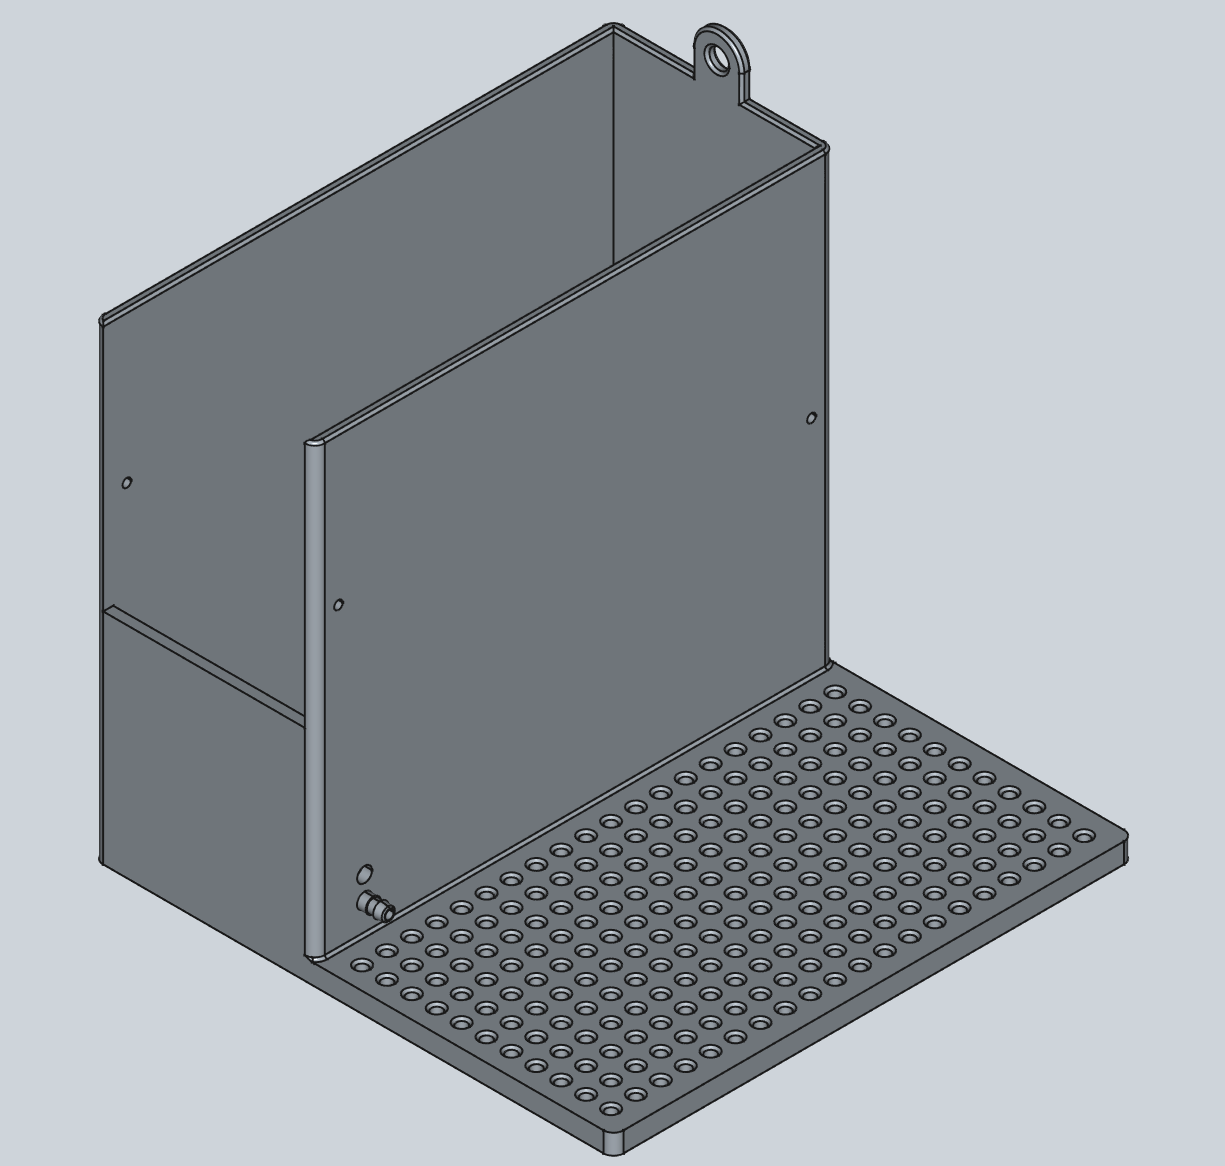
\includegraphics[width=0.8\textwidth]{images/gehaeuse_final.png}
	\caption{Ansicht des finalen Gehäuses}
	\label{fig:gehaeuse}
\end{figure}

Ein weiterer Aspekt, der beachtet werden musste, war die Trennung der elektronischen Komponenten vom Wassergefäß. Deshalb wurde eine Platte an das Gehäuse angesetzt, auf der die Komponenten montiert werden können. Um die einzelnen Bauteile relativ frei platzieren zu können, wurde ein Raster mit einem Lochabstand von 10mm gewählt. In diesem Abstand können nun beliebig Einschmelz-Gewinde mit M3 Gewinde eingesetzt werden. Am tiefsten Punkt des Gehäuses wurde außerdem ein direkter Anschluss für den Wasserschlauch vorgesehen, um den Schlauch nicht über die Wände des Gefäßes führen zu müssen. Das gleiche wurde auch für den Temperatursensor vorgesehen, der dann die Wassertemperatur zum Kühlen überwacht. Gekühlt werden kann die Bierflasche mit kaltem Wasser oder mit Eiswasser. Dafür wurde ein einfaches Loch mit 6mm Durchmesser in der Wand des Gefäß gezeichnet. Um Leckagen am Schlauchanschluss und am Temperatursensor möglichst zu vermeiden, wurde bei der Montage Silikon verwendet. Bei ersten Testdrucken konnten alle Fehler wie die Höhe des Gehäuses oder die Schlauchanbindung oben am Gehäuse, welche zu klein war, beseitigt werden. Der Fehler, der jedoch nicht in der Zeichnung behoben werden konnte, war die Dichtigkeit des Gehäuses an sich. Dieser konnte mit Einstellungen vom 3D-Druck behoben werden.

Dies ist ein guter Zeitpunkt, sich mit den Aspekten des 3D-Drucks an sich zu befassen. Da wäre zum Einen die Materialwahl. Zunächst wurde mit PLA gedruckt, welches das Standardmaterial für den FDM-Druck ist. Es ist einfach zu drucken, jedoch nicht so temperatur- und wasserbeständig wie beispielsweise PETG. PETG lässt sich allerdings nicht so einfach drucken wie PLA und bei Testdrucken konnten keine wasserdichten Gefäße produziert werden. Weitere Materialien wie ABS und ASA sind deutlich beständiger gegenüber äußeren Einflüssen, jedoch auch deutlich teurer als PLA und PETG. Als die Probleme mit der Dichtigkeit auftraten, wurde auch bedacht, mit PETG zu drucken. Dies wurde aber nach weiterer Recherche wieder verworfen, da mit der Erhöhung der Wandstärke und Einstellung diverser Druckparameter ein dichtes Gehäuse gefertigt werden konnte. Das Fertigungsverfahren des 3D-Drucks wurde im Allgemeinen gewählt, da es zur Verfügung stand, ausreichend Präzision bietet und außerdem für Prototyping perfekt ist, um schnell Tests mit den fertigen Bauteilen durchzuführen.

Die Abmessungen des Gehäuses waren durch die Abmaße einer 0,5l Bierflasche relativ schnell festgelegt. Außerdem war der Bauraum des 3D-Druckers mit 256x256x256mm auch ein begrenzender Faktor bei den Abmessungen.

\section{Insert}

Das mechanische Herzstück des Bierkühlers ist der Insert. Er hält die Wellen, auf denen die Flasche gedreht wird, und ist somit strukturell sehr wichtig. Der Insert wird in das Gehäuse eingesetzt, um so möglichst alles an Spritzwasser aufzufangen.

\begin{figure}[htbp]
	\centering
% Dateipfad zum Bild des Inserts hier eintragen
	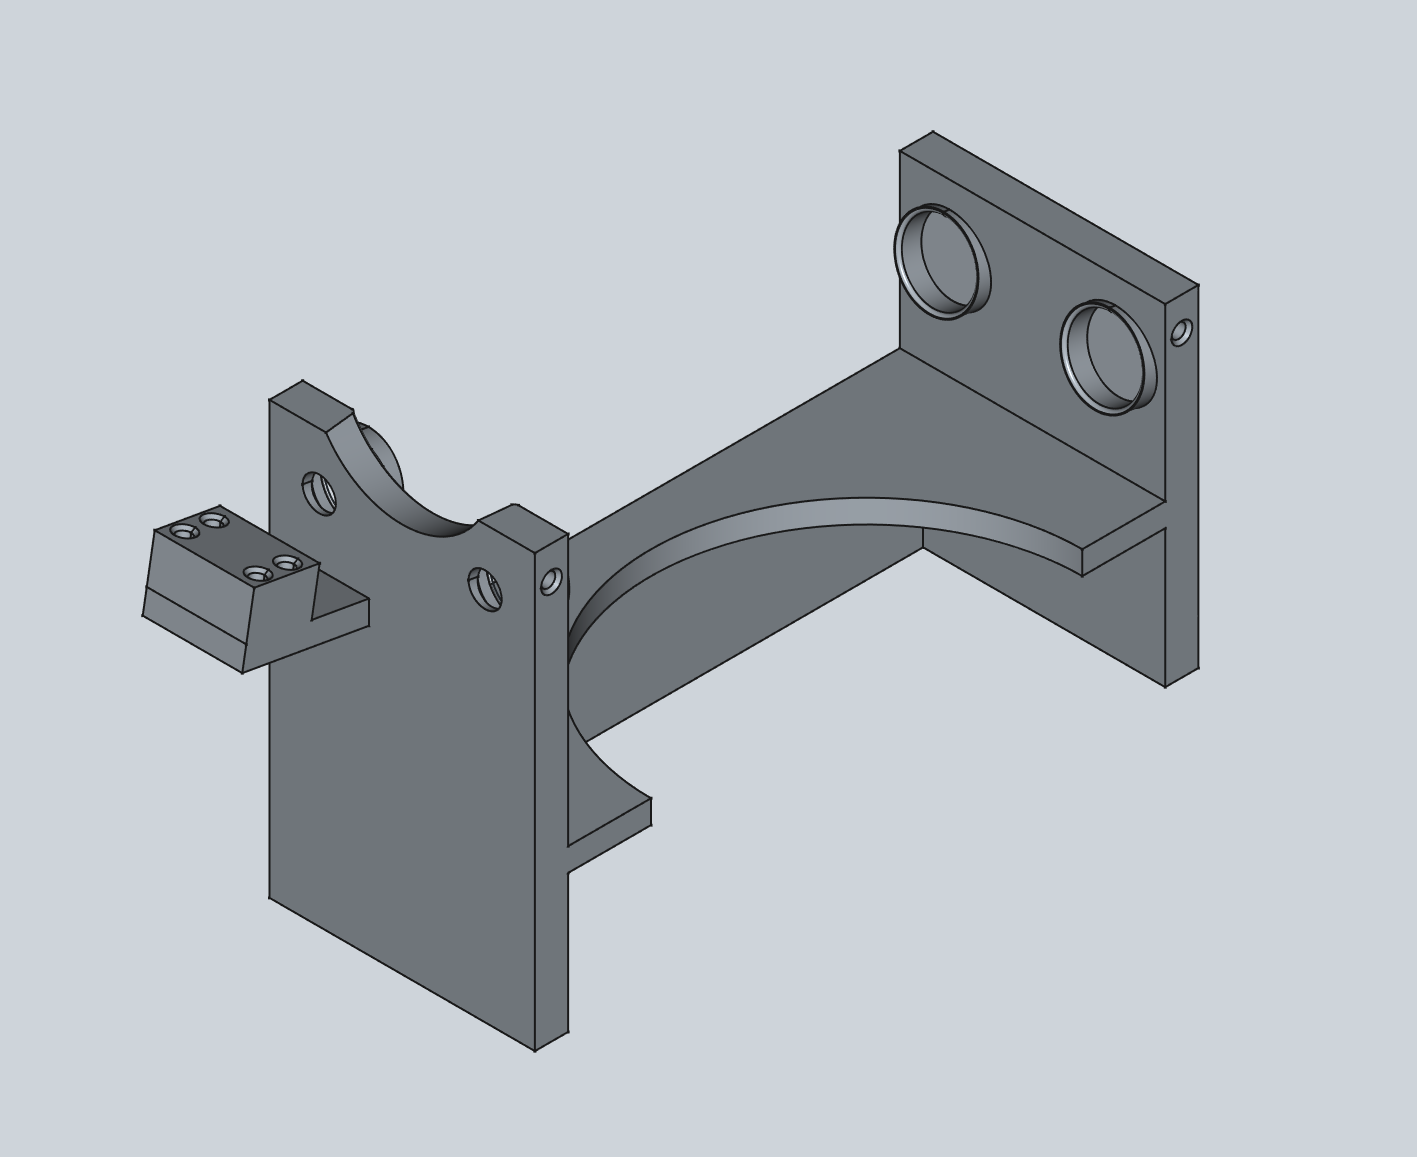
\includegraphics[width=0.8\textwidth]{images/insert.png}
	\caption{Darstellung des mechanischen Inserts}
	\label{fig:insert}
\end{figure}

Der Winkel von 10 Grad, in dem viele Bestandteile des Inserts angeordnet sind, ist damit zu begründen, dass das Wasser nicht in die Richtung des Motors fließt und ihn so beschädigen kann. Ein zu steiler Winkel lässt außerdem das kalte Wasser zu schnell von der Flasche laufen. Bei einem zu kleinen Winkel bleibt das Wasser nur punktuell an der Flasche. Um die Wellen möglichst reibungsfrei drehen zu können, wurden Kugellager vorgesehen. Auf der höheren Seite des Inserts sind Löcher vorgesehen, um daraus die Anbindung an der Welle herauszuführen. Die Anbindung für den Motor wurde mit einem “Balkon” sichergestellt. Die Herausforderung dabei war, die richtige Höhe und Position des "Balkons" zu ermitteln, damit die Welle des Motors direkt auf die Aufnahme an der Welle trifft. Der Motor wird mittels 4 M3 Schrauben am Insert befestigt und die Kugellager können einfach von Hand in das Insert gepresst werden. An der oberen Seite des Inserts ist ein halbrunder Ausschnitt vorgesehen, um so Raum für den Flaschenhals zu gewährleisten. Der Steg zwischen den beiden vertikalen Wänden ist eine Markierung für den richtigen Füllstand des Wassers. Der halbrunde Ausschnitt ist für das Einfüllen des Wassers gedacht. Nach ersten Druckttests konnte festgestellt werden, dass der Insert sich leicht durchbiegen lässt und bei mechanischer Belastung durch eine Bierflasche zu einem unrunden Lauf der Bierflasche selbst geführt hat. Deshalb wurde noch eine zusätzliche Wand zwischen den zwei vertikalen Wänden hinzugefügt. Um das Insert in dem Gehäuse zu fixieren und auch um ein Aufschwimmen des Inserts durch das eingefüllte Wasser zu verhindern, wurden seitlich vier M3 Gewinde vorgesehen. Mit diesen kann der Insert von außerhalb des Gehäuses befestigt werden.

\section{Welle}

Die Wellen sind ein weiterer wichtiger Bestandteil. Auf ihnen wird die Bierflasche gedreht.

\begin{figure}[htbp]
	\centering
% Dateipfad zum Bild der Welle hier eintragen
	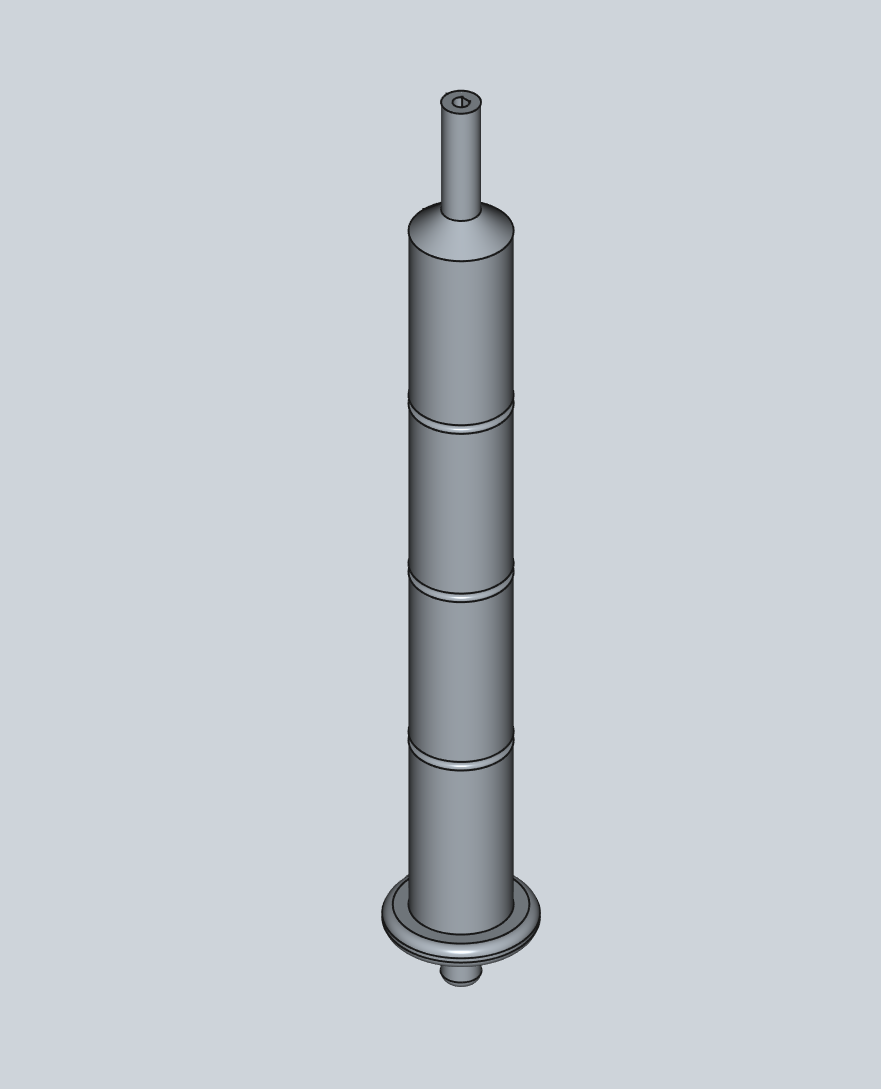
\includegraphics[width=0.8\textwidth]{images/welle.png}
	\caption{Konstruktion der Welle}
	\label{fig:welle}
\end{figure}

Die Durchmesser des oberen und unteren Teils der Welle sind so ausgelegt, dass sie sauber in die Kugellager passen. Im unteren Teil der Welle befindet sich ein Teller, der dafür sorgt, dass die Bierflasche nicht nach unten rutscht und so an anderen Bauteilen schleift. Dabei ist die Größe des Tellers durch die Breite des Inserts und des Gehäuses begrenzt. An der Spitze der Welle ist eine Aufnahme für die Motorwelle vorgesehen. Nach ersten Tests mit der entworfenen Welle konnte beobachtet werden, dass die Welle aufgrund zu geringer Reibung durchdreht und die Flasche nicht sauber mitgedreht wird. Deshalb wurden Rillen in der Welle vorgesehen, in die dann Gummidichtringe gesetzt werden können. Mit diesen konnte die Reibung erhöht werden und die Flasche dreht sich mit der Welle. Ein weiteres Maß, welches beeinflusst werden konnte, war der Durchmesser der Welle. Zunächst war ein Durchmesser von 2cm vorgesehen. Da der Motor mit 100 Umdrehungen pro Minute relativ schnell dreht, war es notwendig, den Durchmesser auf 1cm zu verringern. So konnte eine Reduzierung der Geschwindigkeit der Flasche auf die Hälfte sichergestellt werden. Aufgrund der verschiedenen Flaschenformen fiel bei Tests zunächst nicht auf, dass der Flaschenhals am Insert schliff. Deshalb musste der Durchmesser wieder erhöht werden. Um dem zu schnellen Drehen der Flasche entgegenzuwirken, wurden PWM-Signale zur Motoransteuerung verwendet, um die Drehzahl des Motors zu senken. Aufgrund des hohen Moments des Motors trat bei weiteren Tests eine Ermüdung der Aufnahme auf. Dabei drehte sich der Motor ohne die Welle mitzunehmen. Um diesem Verhalten vorzubeugen, wurde die Antriebswelle mit Sekundenkleber in der Welle befestigt.

\section{Abdeckung}

Um den Bereich am Wasserauslass besser vor Spritzwasser zu schützen, wurde eine Abdeckung für den hinteren Bereich entworfen. Außerdem können dabei auch die Bedienelemente so befestigt werden, dass sie leicht erreichbar sind.

\begin{figure}[htbp]
	\centering
% Dateipfad zum Bild der Abdeckung hier eintragen
	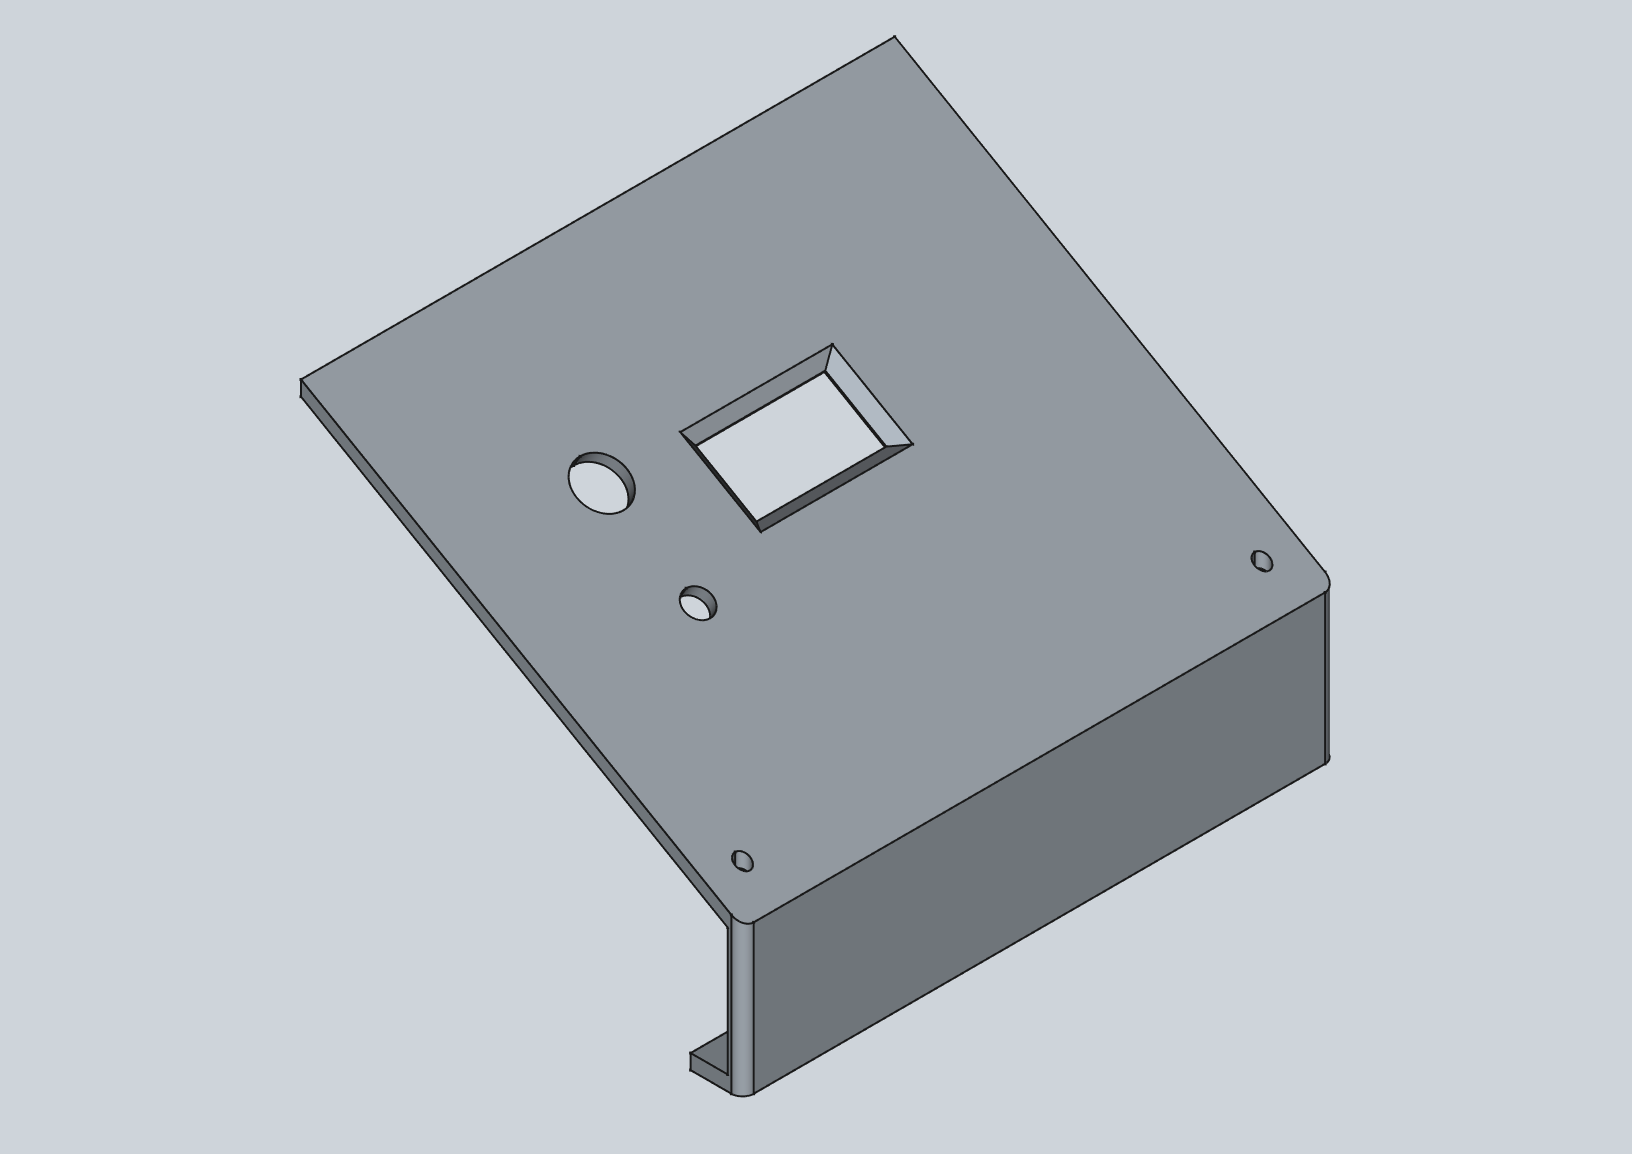
\includegraphics[width=0.8\textwidth]{images/abdeckung.png}
	\caption{Abdeckung und Bedienelemente}
	\label{fig:abdeckung}
\end{figure}

Um die Abdeckung zu montieren, wurden Löcher an der Unterseite der Abdeckung vorgesehen, die mit dem Raster am Gehäuse übereinstimmen. Der Winkel der Abdeckung wurde so gewählt, dass das Display gut abzulesen ist. Der Rotary Encoder und der Knopf können durch einfache Bohrungen an der Abdeckung befestigt werden. Für das Display wurde ein rechteckiger Ausschnitt vorgesehen. Die Phase um das Display wurde aus ästhetischen Gründen hinzugefügt. Für die Befestigung des Displays wurden vier Dome im Abstand der Schraublöcher auf der Innenseite des Gehäuses erstellt mit einem größeren Durchmesser als die Löcher des Displays. Auf den vier Domen zur Fixierung der Displayposition wurden je eine Verjüngung hinzugefügt, die einen kleineren Durchmesser als die Löcher des Displays aufweisen. Nach der Montage bzw. Fixierung des Displays kann man die Verjüngung mit einem Lötkolben verschmolzen. Das verschmolzene Material sorgt dann dafür, dass das Display ohne Schrauben fixiert werden kann. Die Abdeckung ist so breit wie die Platte, sodass sie direkt am Gehäuse anliegt.

\section{Montageaufnahmen}

Um die verschiedenen Komponenten zu befestigen, wurden einige Aufnahmen benötigt. Da Teile wie der Spannungswandler, der Mikrocontroller oder die PWM-Module Standardbauteile sind, die häufig für Elektronikbasteleien verwendet werden, konnten dafür bereits existierende Aufnahmen und Gehäuse genutzt werden, welche unter Thingiverse oder Makerworld veröffentlicht wurden. Diese hatten meist nicht die passenden Schraublöcher, um auf dem Raster montiert zu werden. Deshalb wurden die Gehäuse gedruckt und anschließend Löcher im Rastermaß gebohrt.

\begin{figure}[htbp]
	\centering
	% Drei Bilder nebeneinander (zusammen < 1 \textwidth, damit sie in eine Zeile passen)
	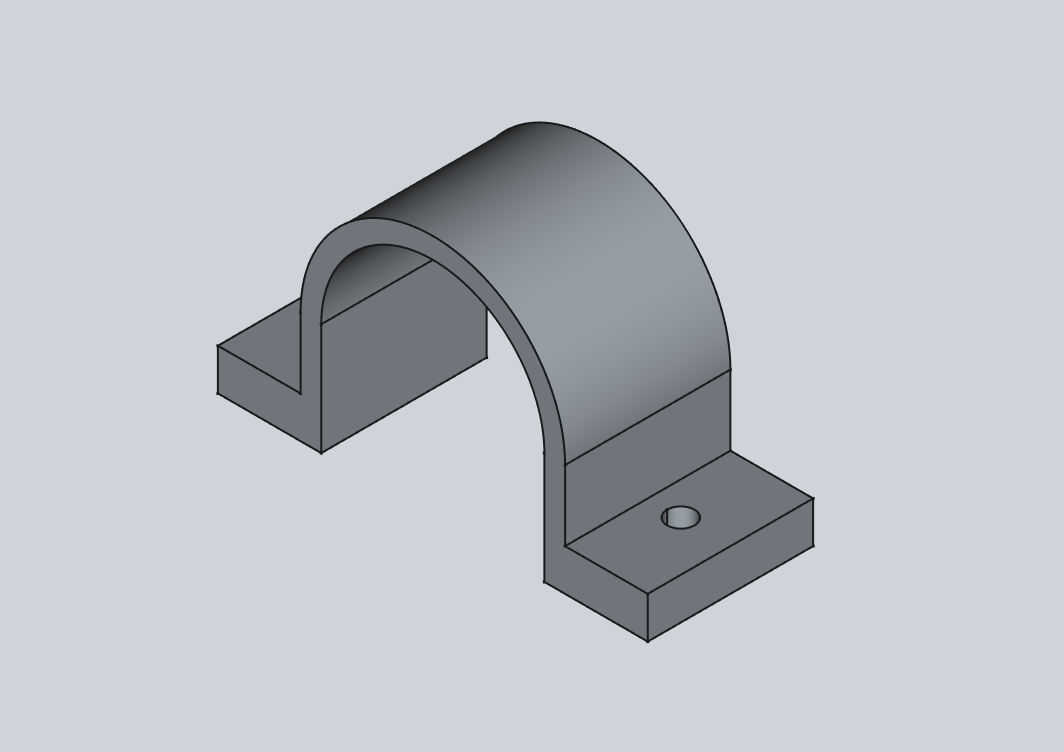
\includegraphics[width=0.32\textwidth]{images/klemme1.png}\hfill
	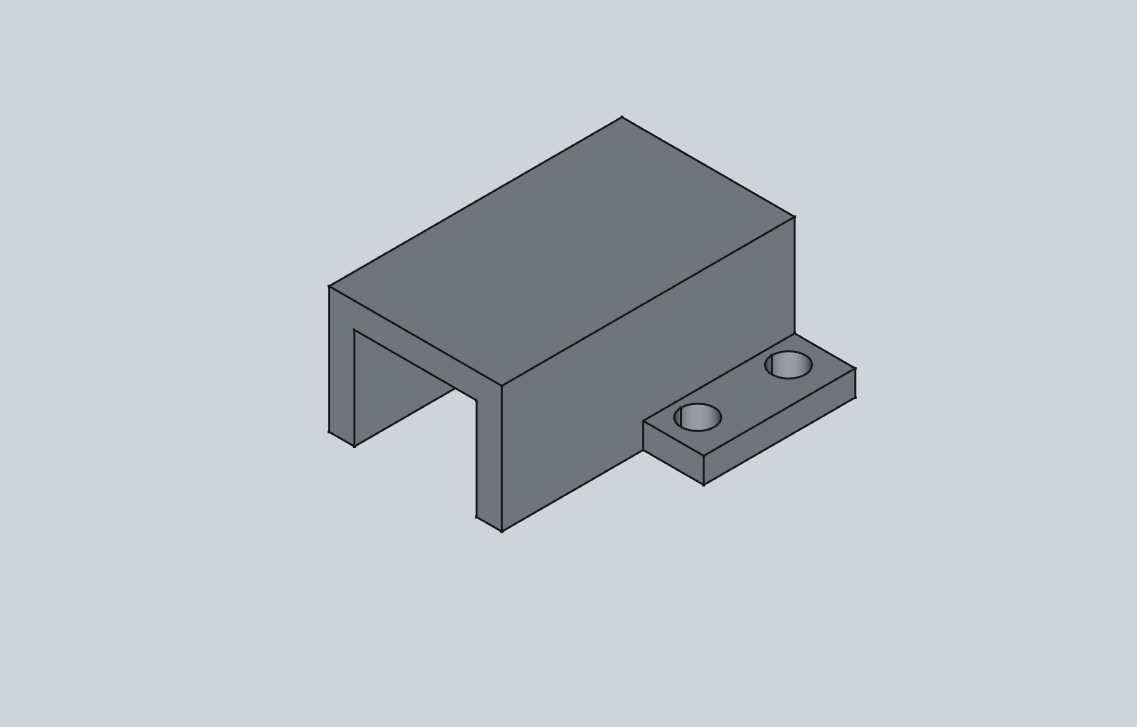
\includegraphics[width=0.32\textwidth]{images/klemme2.png}\hfill
	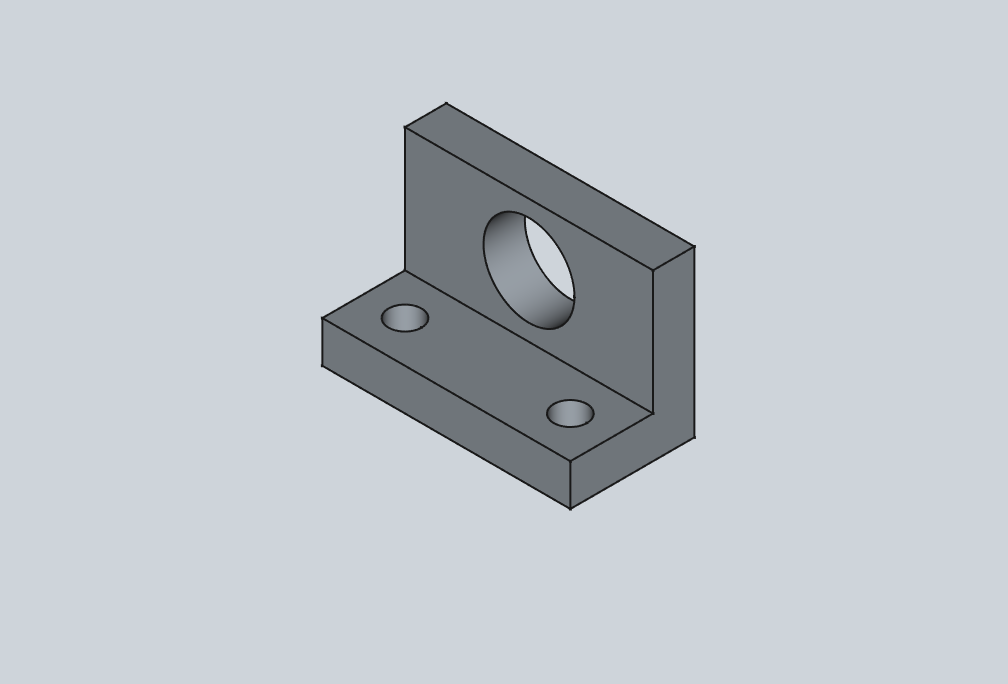
\includegraphics[width=0.32\textwidth]{images/klemme3.png}
	
	\caption{Montageaufnahmen für die Komponenten}
	\label{fig:montageaufnahmen}
\end{figure}

Für den Motor wurde eine Halterung gezeichnet, die genau auf den “Balkon” des Insert passt und die dort vorgesehenen Schraublöcher nutzt. Außerdem ist die Abdeckung extra etwas länger als der Motor, um den Motor besser vor Spritzwasser zu schützen. Für die Pumpe wurde eine Klemme designt, welche die Pumpe an ihrer breitesten Stelle eingeklemmt. Die Aufnahme wurde neben dem Auslass am Gehäuse montiert. Um keinen Knick im Schlauch zu provozieren, wurde ein 90 Grad Winkel in der passenden Größe verwendet. Für die Aufnahme des Hohlsteckers (5.5mm x 2.1mm) zur Kontaktierung mit dem Steckernetzteil wurde ein einfacher Winkel mit einer Bohrung für die Buchse entworfen. Die Aufnahme wurde am hinteren Ende des Gehäuses festgeschraubt. Die restlichen Komponenten wurden an die passenden Stellen platziert, die günstig bei der Verdrahtung waren. Aufgrund der vielen Komponenten wurde außerdem eine Lochrasterplatine mit Stiftleisten zur Verteilung von Ground und 3,3 Volt angefertigt, welche auch auf dem Raster platziert wurde.

\section{Zusammenfassung}

Der mechanische Aufbau des Bierkühlers konnte erfolgreich als funktionsfähiger Prototyp realisiert werden. Durch den konsequenten Einsatz von CAD-Konstruktion in FreeCAD und der additiven Fertigung war es möglich, eine hochgradig integrierte Lösung zu schaffen, die sowohl die fluidtechnischen Anforderungen (Kühlung durch Wasser) als auch die elektromechanischen Vorgaben (Rotation und Sensorik) erfüllt.

Das gewählte Raster-Konzept auf der Montageplatte erwies sich als besonders vorteilhaft, da es eine flexible Positionierung der Steuerungsmodule des STM32 und der Leistungselektronik ermöglichte. Die räumliche Trennung von Nass- und Trockenbereich sorgt für die notwendige Betriebssicherheit des Mikrocontrollers. Durch konstruktive Iterationen an den Wellen und dem Insert konnte ein zuverlässiger Kraftschluss zwischen Motor und Kühlgut sichergestellt werden, während die Abdichtung des Gehäuses durch eine Optimierung der Druckparameter ohne zusätzliche Werkstoffe realisiert wurde.

